
\newcommand{\nomedoc}{Specifica Tecnica}
\newcommand{\versione}{0.2}
\newcommand{\versioneglossario}{1.0}
\newcommand{\versionenormeprogetto}{1.0}
\newcommand{\nomefile}{SpecificaTecnica-\versione.pdf}
\newcommand{\datacreazione}{2 Dicembre 2010}
\newcommand{\datamodifica}{27 Gennaio 2011}
\newcommand{\stato}{formale}
\newcommand{\uso}{interno}
\newcommand{\redazione}{Mandolo Andrea}
\newcommand{\verifica}{---}
\newcommand{\approvazione}{---}
\newcommand{\distribuzione}{
VT.G \\
& Prof. Vardanega Tullio\\
& Prof. Cardin Riccardo }

% FUNZIONI TIPOGRAFICHE
\newcommand{\co}{\texttt} % courier
\newcommand{\bo}{\textbf} % bold
\newcommand{\pr}{\par\medskip} % paragrafo spaziato
\newcommand{\sca}{\textsc} % small caps

\documentclass[a4paper,12pt]{report}
% 10pt,11pt,12pt
% titlepage, notitlepage -> per dare inizio o no ad una nuova pagina dopo titolo
% twoside -> per dire se fronte-retro
\usepackage[latin1]{inputenc}
% per caratteri accentati
\usepackage[italian]{babel}
% per regole sintattiche italiane
\usepackage[bookmarks=true, pdfborder={0 0 0 0}]{hyperref}
% per collegamenti ipertestuali
\usepackage{graphicx}
% per inserimento immagini

% \usepackage{enumerate}
% per personalizzare elenchi puntati

\usepackage[hmargin=2cm]{geometry} %margine 2 cm
%\geometry{options varie}

% comandi per gestire meglio header e footer
\usepackage{fancyhdr}  % header e footer
\usepackage{totpages}
\pagestyle{fancy}
\renewcommand{\headrulewidth}{0.4pt}
\renewcommand{\footrulewidth}{0.4pt}

\setlength{\headheight}{1.2cm} % NON TOCCARE
\setlength{\voffset}{-1.5cm} % NON TOCCARE
\setlength{\textheight}{666pt} % NON TOCCARE
\setlength{\footskip}{60pt}
\setlength{\parindent}{0pt} % INDENTAZIONE

\lhead{\nomedoc\  (ver. \versione)}
\chead{}
\rhead{
\includegraphics[height=1cm]{img/netmus.png}}
\lfoot{
\includegraphics[height=0.8cm]{img/logo.png}}
\cfoot{}
\rfoot{\thepage}

\usepackage{titlesec}
\titleformat{\chapter}{\normalfont\huge\bfseries}
{\thechapter}{20pt}{\Huge}

\usepackage{rotating}   % PER TABELLE E AMBIENTI RUOTATI
\usepackage{array}
\usepackage{color}
\usepackage{colortbl}  % VARIE PER GESTIRE I COLORI
\definecolor{Orange}{RGB}{255,127,0}   % ARANCIO ACCES0
\definecolor{orange}{RGB}{255,207,80}  % ARANCIO TENUE

\addtocontents{toc}{\protect\thispagestyle{fancy}}  % PER INDICI CON + PAGINE
\usepackage[font=it]{caption}    % PER RENDERE CORSIVE LE DIDASCALIE
\usepackage{eurosym}  % PER SIMBOLO EURO

% \usepackage{listings}   per codice sorgente

\author{VT.G - Valter Texas Group}

\begin{document}

\pagenumbering{Roman} % INIZIO NUMERAZIONE ARABA

\vspace*{1cm}
\begin{center}

\begin{LARGE} \sca{Federico Baron} \end{LARGE}\\
\vspace{0.5cm}
\begin{Large}
\emph{fede.baron.89@gmail.com} \end{Large}\\
\vspace*{1cm} 
\includegraphics[width=5cm]{img/logo.png}\\
\vspace{0.5cm}
\begin{Large} \emph{``Comunicazione Aumentata/Alternativa per Giovani Ospiti
della Terapia Intensiva Pediatrica''} \end{Large}\\
\vspace{3cm}
\begin{Large} \sca{\nomedoc} \end{Large}\\
\end{center}
\vspace{1cm}

% INFORMAZIONI DOCUMENTO
\begin{center}
\begin{tabular}{r|l}
\hline & \\
\bo{Nome} & \nomefile \\
\bo{Versione attuale} & \versione \\
\bo{Data creazione} & \datacreazione \\
\bo{Data ultima modifica} & \datamodifica \\
\bo{Redazione} & \redazione \\
& \\\hline
\end{tabular}
\end{center}
\newpage

% REGISTRO MODIFICHE
\section*{Registro delle modifiche}

\begin{longtable}{|p{0.13\textwidth}|c|p{0.2\textwidth}|p{0.46\textwidth}|}
\hline
\rowcolor{orange} \bo{Data} & \bo{Versione} & \bo{Autore} & \bo{Descrizione} \\
\hline
\endhead
\hline
\endfoot

27/01/2011 & 0.2 & Mandolo Andrea & Inserita presentazione dell'architettura
generale del sistema.\\
\hline
21/01/2011 & 0.1 & Mandolo Andrea & Creato documento iniziale.\\

\end{longtable}

% INDICE
\tableofcontents

\chapter*{Sommario}
-- da compilare --


\thispagestyle{fancy} % serve perche' nelle pagine di inizio Chapter esca header e footer
\pagenumbering{arabic} % INIZIO NUMERAZIONE NORMALE
\rfoot{\thepage\ di \pageref{TotPages}}
\addcontentsline{toc}{chapter}{Sommario}

\chapter{Introduzione}
\thispagestyle{fancy} % serve perche' nelle pagine di inizio Chapter esca header e footer

\section{Scopo del documento}
Lo scopo della Specifica Tecnica \`e quello di illustrare le scelte progettuali
che il gruppo ha deciso di seguire nella realizzazione del prodotto. Viene
presentata, pur restando ad alto livello, la gerarchia dei package, delle loro
connessioni e delle principali classi di cui essi si compongono.


\section{Scopo del prodotto}
Il progetto \underline{NetMus} nasce con lo scopo di realizzare un sistema
software basato su \underline{cloud} \underline{computing}, per memorizzare
informazioni di brani musicali in profili utente online.\\ Tali informazioni vengono estratte da
dispositivi musicali o di archiviazione \underline{USB} al momento della loro connessione.

\section{Glossario}
Il Glossario \`e definito con un documento a parte
(\emph{Glossario-\versioneglossario.pdf}). Tutti i termini caratterizzati da
\underline{questa sottolineatura} sono ivi definiti.\\
Verr\`a sottolineata solamente la prima occorrenza di ciascun
termine presente nel Glossario, per non compromettere la leggibilit\`a del documento.

\section{Riferimenti}

\subsection{Normativi} % oppure rif. a Norme di progetto con leggi e tutto
\begin{itemize}
  \item ISO/IEC 12207:1995 - Cicli di vita software
  \item ISO/IEC 9126:2001 - Quality Model
  \item \emph{NormeDiProgetto-\versionenormeprogetto.pdf} che regola e
  accompagna tutti i documenti ufficiali.
\end{itemize}
\newpage
\subsection{Informativi}
\begin{itemize}
  \item Capitolato d'appalto CO2-NETMUS del corso di Ingegneria del Software
  A.A. 2010/11 :\\
  \url{http://www.math.unipd.it/~tullio/IS-1/2010/Progetto/NetMus.pdf}
  \item Slide delle lezioni del corso:\\
  \url{http://www.math.unipd.it/~tullio/IS-1/2010/}
  \item Verbale intervista proponente:\\
  \co{allegato Verbale-1.0.pdf}
  \item Sistema di cloud Google App Engine:\\
  \url{http://code.google.com/intl/it/appengine/}
\end{itemize}


\chapter{Definizione del Prodotto}
\section{Metodo e formalismo di specifica}

\section{Presentazione dell'architettura generale del sistema.}

Il sistema Netmus sar\`a principalmente formato dai seguenti package:
\begin{figure}[h]
  \centering
  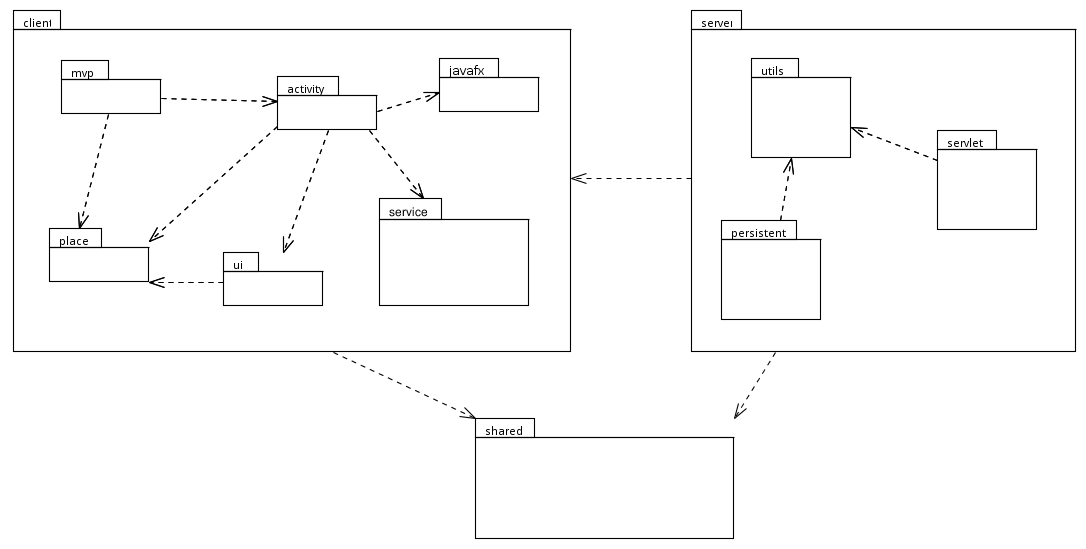
\includegraphics[width=16cm]{img/ST/PackageGeneric.png}
\caption{Diagramma dei package principali di Netmus.}
\end{figure}

\begin{itemize}
  \item Package \emph{client} : definisce la parte client del programma
  \begin {itemize}
    \item Package \emph{client::ui} : comprende l'insieme di viste del sistema,
    rispettando il framework \emph{MVP with Place and Activity}. Ci sar\`a una
    interfaccia per ogni vista, per dare la possibilit\`a di creare in futuro
    pi\`u implementazioni differenti a seconda del dispositivo client;
    \item Package \emph{client::activity} : rappresenta l'insieme di classi
    controllori che formano la logica del sistema. Esse mandano dati aggiornati alle
    viste, gestiscono le richieste delle viste e possono inoltre gestire
    richieste provenienti da altre componenti e mandare eventi propri nell'event-bus;
    \item Package \emph{client::place} : comprende l'insieme di classi Place i
    quali rappresentano un URL associato ad una vista. Gestiscono i parametri
    agganciati all'URL con un Tokenizer interno;
    \item Package \emph{client::mvp} : comprende un ActivityMapper e
    un PlaceHistoryManager che mappano per ogni Place la sua corrispondente
    Activity e gestiscono la cronologia dei Place;
    \item Package \emph{client::service} : rappresenta l'insieme di interfaccie
    che offrono un servizio di comunicazione col server tramite GWT RPC;
    %----------------- TOGLIERE FORSE --------------------
    \item Package \emph{client::javafx} : contiene l'interfacciamento alla
    applet JavaFX di estrazione dei TAG dagli Mp3 da dispositivi multimediali del client;
    %-------------------------------------------------------
  \end {itemize}
  \item Package \emph{server} : rappresenta la parte server di Netmus
  \begin{itemize}
    \item Package \emph{server::persistent} : comprende tutte le classi che
    rappresentano un entit\`a JDO (Java Data Object), le quali usate per lo scambio dati tra
    server e Google Datastore;
    \item Package \emph{server::servlet} : comprende tutte le servlet utilizzate
    per interfacciarsi a servizi esterni (es. Google Authentication, YouTube);
    \item Package \emph{server::utils} : comprende classi di utilit\`a per
    svolgere attivit\`a interne al server di varie tipologie;
  \end{itemize}
  \item Package \emph{shared} :  contiene classi condivise tra client e server,
  che verrano anch'esse compilate in JavaScript da GWT, come tutto il package
  client. La maggior parte saranno gli oggetti di trasferimento che
  aderiscono al pattern DTO.
\end{itemize}


\chapter{Descrizione dei singoli componenti}
\section{Package client}
\begin{figure}[h]
  \centering
  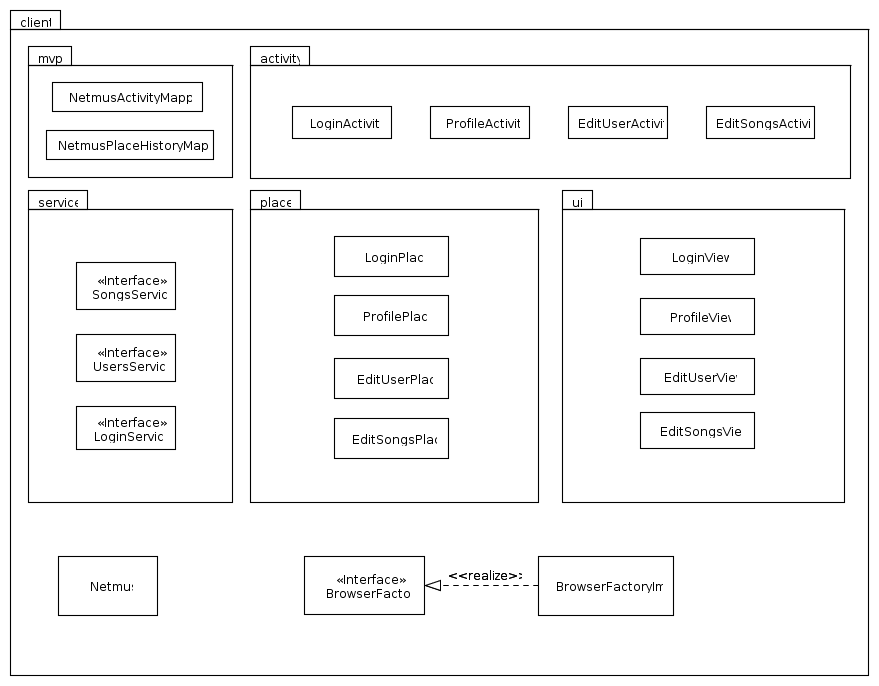
\includegraphics[width=16cm]{img/ST/ClassClient.png}
\caption{Diagramma delle classi del package client.}
\end{figure}

\subsection{Tipo, obiettivo e funzione del componente}
\subsection{Relazioni d'uso di altre componenti}
\subsection{Interfacce con e relazioni di uso da altre componenti}
\subsection{Attivit\`a svolte e dati trattati}

\chapter{Stime di fattibilit\`a e di bisogno di risorse}

\chapter{Tracciamento della relazione componenti - requisiti}

\end{document}
